\subsection{g}
Kombiniert man nun die Werte für die Kollektorfläche und den Durchfluss im Kollektorkreis, kann man
mittels des in \autoref{fig:Druckverlust} vom Hersteller gegebenen Diagrammes den Druckverlust
über einen Kollektor und damit auch
den Druckverlust des Kollektorfeldes in unterschiedlichen Verschaltungen berechnen. Für eine vollkommende
Parallelschaltung der 8 Kollektoren ergibt sich demnach ein Druckverlust von 14500 Pa.
Verglichen mit einer Parallelschaltung von zwei Reihenschaltungen á 4 Kollektoren, welche dann einen
Druckverlust von 58000 Pa vorweisen würde, ist die Parallelschaltung aller 8 Kollektoren deutlich verlustärmer, weshalb im Weiteren
von diesem Fall ausgegangen wird.
\begin{figure}[H]
    \centering
    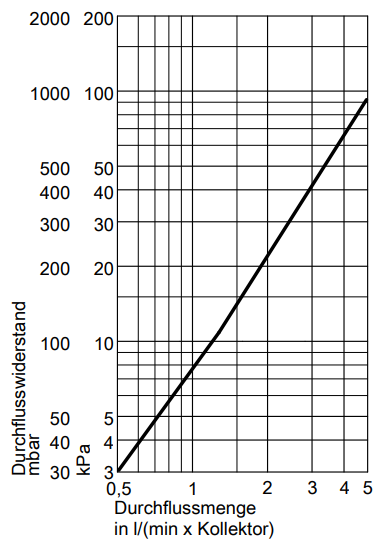
\includegraphics[width=0.65\textwidth]{Abbildungen/Druckverlust.png}
    \caption{Durchflusswiderstand Vitosol-FM/-F, Typ SV und SH\cite[S.129]{Viessmann}}
    \label{fig:Druckverlust}  
\end{figure}
